\documentclass[12pt]{extarticle}

\usepackage[english]{babel}% Idioma español, "es-tabla" para que cambiar el caption "cuadro" por "tabla"
\usepackage[latin1]{}
\usepackage[utf8x]{inputenc}

% Márgenes-------------------------------------------------------
\usepackage[a4paper, paperwidth=21cm, paperheight=29.7cm, top=2.4cm, bottom=2.4cm, left=1.5cm, right=1.5cm]{geometry}
\parindent=0mm
\renewcommand{\baselinestretch}{1.1} %{1.5} genera un texto a espacio y medio. Si se pone 2, lo hace a doble espacio.
%------------------------------------------------------------------------------------------------------------------------------

%-----------------------------------------------------------------------------------------------------
%justificar sin dividir las palabras
%-----------------------------------------------------------------------------------------------------

\tolerance=1
\emergencystretch=\maxdimen
\hyphenpenalty=10000
\hbadness=10000
%----------------------------------------------------------------------------------------------------- 

\usepackage[titles]{tocloft}
\usepackage{amsthm} 
\pagenumbering{roman}
\usepackage{times}
\usepackage{subfig}
\usepackage{fancyhdr}
\usepackage{setspace}
\usepackage{shadow}
\usepackage{fancybox}
\usepackage{eepic}
\usepackage{ifpdf}
\usepackage{pdflscape}
\usepackage{lineno}%numerrar lineas para revision
\usepackage{titlesec}
% \usepackage[none]{hyphenat}%no dividir las palabras por sílabas
\usepackage{ragged2e}%justificar el texto:->\justifying

%----------------------------------------------------------------------------------------------------------------------------
% \usepackage{chngcntr}
% \counterwithout{figure}{chapter}
% \counterwithout{table}{section}
%------------------------------------------------------------------------------------------------------------------------------
% \linenumbers %Numeracion de los renglones para revision
%--------------------------------------------------------------------------------------------------------------------------------------

% Otros paquetes --------------------------------------------------
\usepackage{mathpazo} %fuente palatino
\usepackage[dvips]{graphicx}			      %Soporte para gráficos.
\DeclareGraphicsExtensions{.pdf,.png,.jpg}
\DeclareGraphicsRule{.wmf}{bmp}{}{}
\usepackage{graphics,setspace}
\usepackage{color,soul}
\usepackage[usenames,dvipsnames,svgnames,table]{xcolor}
% \usepackage{pdftricks}%{\blue AZUL} produce AZUL en color azul
\usepackage[T1]{fontenc}
\usepackage{latexsym,amsmath,amssymb,amsfonts,cancel}
\usepackage{multirow, array} % para las tablas
\usepackage{dcolumn}
\usepackage{booktabs}
\usepackage{float} % para usar [H]
\usepackage{enumitem}
\usepackage{caption}
\captionsetup{font=small,labelfont=bf}
\usepackage{multicol}
\usepackage{sidecap}
\usepackage{wrapfig}%%%%%%%%%figuras en dos columnas
\usepackage{epstopdf}
\usepackage[tc]{titlepic}
% \usepackage{makeidx} %If you want to generate an index, automatically 
% Referencias - ligas
\usepackage{url}
\usepackage[bookmarks=true,linktoc=page,breaklinks,colorlinks=true, pdfstartview=FitV, linkcolor=azul, urlcolor=gris, anchorcolor=azul, citecolor=rojo,colorlinks=true,pdfborderstyle={/S/U/W 1}]{hyperref}
\usepackage{hyperref}
\usepackage[square,compress,comma,numbers,super]{natbib}% superindice los números de las referencias \cite{} !!!!conflictos con cite package



%#####----natbib option-----##########
% round: (default) for round parentheses;
% square: for square brackets;
% curly: for curly braces;
% angle: for angle brackets;
% colon: (default) to separate multiple citations with colons;
% comma: to use commas as separaters;
% authoryear: (default) for author-year citations;
% numbers: for numerical citations;
% super: for superscripted numerical citations, as in Nature;
% sort: orders multiple citations into the sequence in which they appear in the list of references;
% sort&compress: as sort but in addition multiple numerical citations are compressed if possible (as 3-6, 15);
% longnamesfirst: makes the first citation of any reference the equivalent of the starred variant (full author list) and subsequent citations normal (abbreviated list);
% sectionbib: redefines \thebibliography to issue \textbf* instead of \chapter*; valid only for classes with a \chapter command; to be used with the chapterbib package;
% nonamebreak: keeps all the authors' names in a citation on one line; causes overfull hboxes but helps with some hyperref problems.
%######------------------#################

% \usepackage[super]{cite}%conflictos con natbib package

\usepackage{tikz}
\usepackage{afterpage}%color page



\usepackage{lipsum} % filler text
\usepackage{etoolbox}
\usepackage{fancyhdr}
% \pagestyle{fancy}%nombra la secciones y las subsecciones en el encabezado del texto	
% \usepackage[nottoc,numbib]{tocbibind}%remove the self-reference of the ToC 
%----------------------------------------------------------------------------------------------------------------------------
%Colores
\definecolor{azul}{RGB}{15,140,230}
\definecolor{rojo}{RGB}{233,27,255}
\definecolor{gris}{RGB}{70,70,70}

%----------------------------------------------------------------------------------------------------------------------------


% \setcounter{chapter}{0}

\newcounter{mathematicapage}

%Para corregir lo de los hboxes llenos
\hbadness=100000
\hfuzz=100pt
%error \vbox (badness 10000)...
\makeatletter
 \def\@textbottom{\vskip \z@ \@plus 100pt}
 \let\@texttop\relax
\makeatother
%error headheight is too smal
\setlength{\headheight}{16pt}


%%%%%%%%%%%%%%%%%%%%%%%%%%%%%%
%\renewcommand{\figurename}{Fig.} %Cambia la palabra "Figura" por "Fig."
\renewcommand{\listtablename}{Indice de tablas}
\renewcommand{\tablename}{Tabla.} %Cambia la palabra "Cuadro" por "Tabla"

\renewcommand\thefigure{\arabic{figure}} % Genera numeración Y.
\renewcommand\thetable{\arabic{table}} % Genera numeración Y.

%\renewcommand\thefigure{\arabic{section}.\arabic{figure}.} % Genera numeración X.Y.
%\renewcommand\thetable{\arabic{section}.\arabic{table}.} % Genera numeración X.Y.
%\numberwithin{figure}{section} %Hace que la primera figura de cada sección X sea X.1
%\numberwithin{table}{chapter} %Hace que la primera tabla de cada sección X sea X.1

%%%%%%%%%%%%%%%%%%%%%%%%%%%%%%%%%%%

\renewcommand{\thepage}{\arabic{page}}%numerar en arabicos ####\renewcommand{\thepage}{\roman{page}}

%----------------------------------------------------------------------------------------------------------------------------
%------------------pdf inclusion multiple pdfs
\pdfsuppresswarningpagegroup=1

















%--------------------------------------------------------------------------------------------------------
% \date{}

\pdfinfo{%
  /Title    (Curriculum Vitae EN)
  /Author   (Edison Flórez)
  /Creator  (Edison Flórez)
  /Producer ()
  /Subject  ()
  /Keywords ()
}

\color{gris}
\begin{document}
%--------------------------------------------------------------------------------------------------------
\pagestyle{fancy}
\fancyhf{}
\fancyhead[R]{\textcolor{gray}{\scriptsize Last update \today}} %E for even page O for odd page L for left side C for centered R for right side
% \fancyhead[RE,LO]{Guides and tutorials}
% \fancyfoot[CE,CO]{\leftmark}
\fancyfoot[C]{\thepage}


% \pagecolor{gray!20}\afterpage{\nopagecolor}
% \colorbox{gray!20!white}{
\begin{minipage}{0.32\columnwidth}

\tikz[remember picture,overlay] \draw [fill,gray!20!white] (current page.north west) rectangle +(0.36\paperwidth,-1.0\paperheight);

\vspace*{-14.25mm}
\noindent
{\color{black!75!white}\rule{1.06\linewidth}{0.15mm} }

 \vspace*{-10mm}
 \begin{flushright}

%   \textcolor{azul}{\bf\Large Address}\\ \vspace*{2.7mm}
% 
%     eCentre, Private Bag 102 904\\ \vspace*{-0.5mm}
%     NZIAS, Massey University\\ \vspace*{-0.5mm}
%     Auckland (0632), NZ
%     \vspace*{4mm}

  \textcolor{azul}{\bf\Large Telephone}\\ \vspace*{3mm}

    (64) 204 1437112 \\ \vspace*{-0.5mm}
    (64) 9 414 0800 ext. 43599\\ 
    \vspace*{4mm}

  \textcolor{azul}{\bf\Large Zoom/Skype}\\ \vspace*{3mm}
  
    edisonffh%@outlook.com\\
    \vspace*{4mm}
    
  \textcolor{azul}{\bf\Large eMail}\\ \vspace*{3mm}

    \href{mailto:edisonffh@gmail.com}{\textbf{edisonffh@}\\[-1mm]gmail.com}\\ 
    \href{mailto:e.florez@massey.ac.nz}{\textbf{e.florez@}\\[-2mm]massey.ac.nz}\\
    \vspace*{6mm}

  \textcolor{azul}{\bf\Large Key Skills}\\ %\vspace*{3mm}
   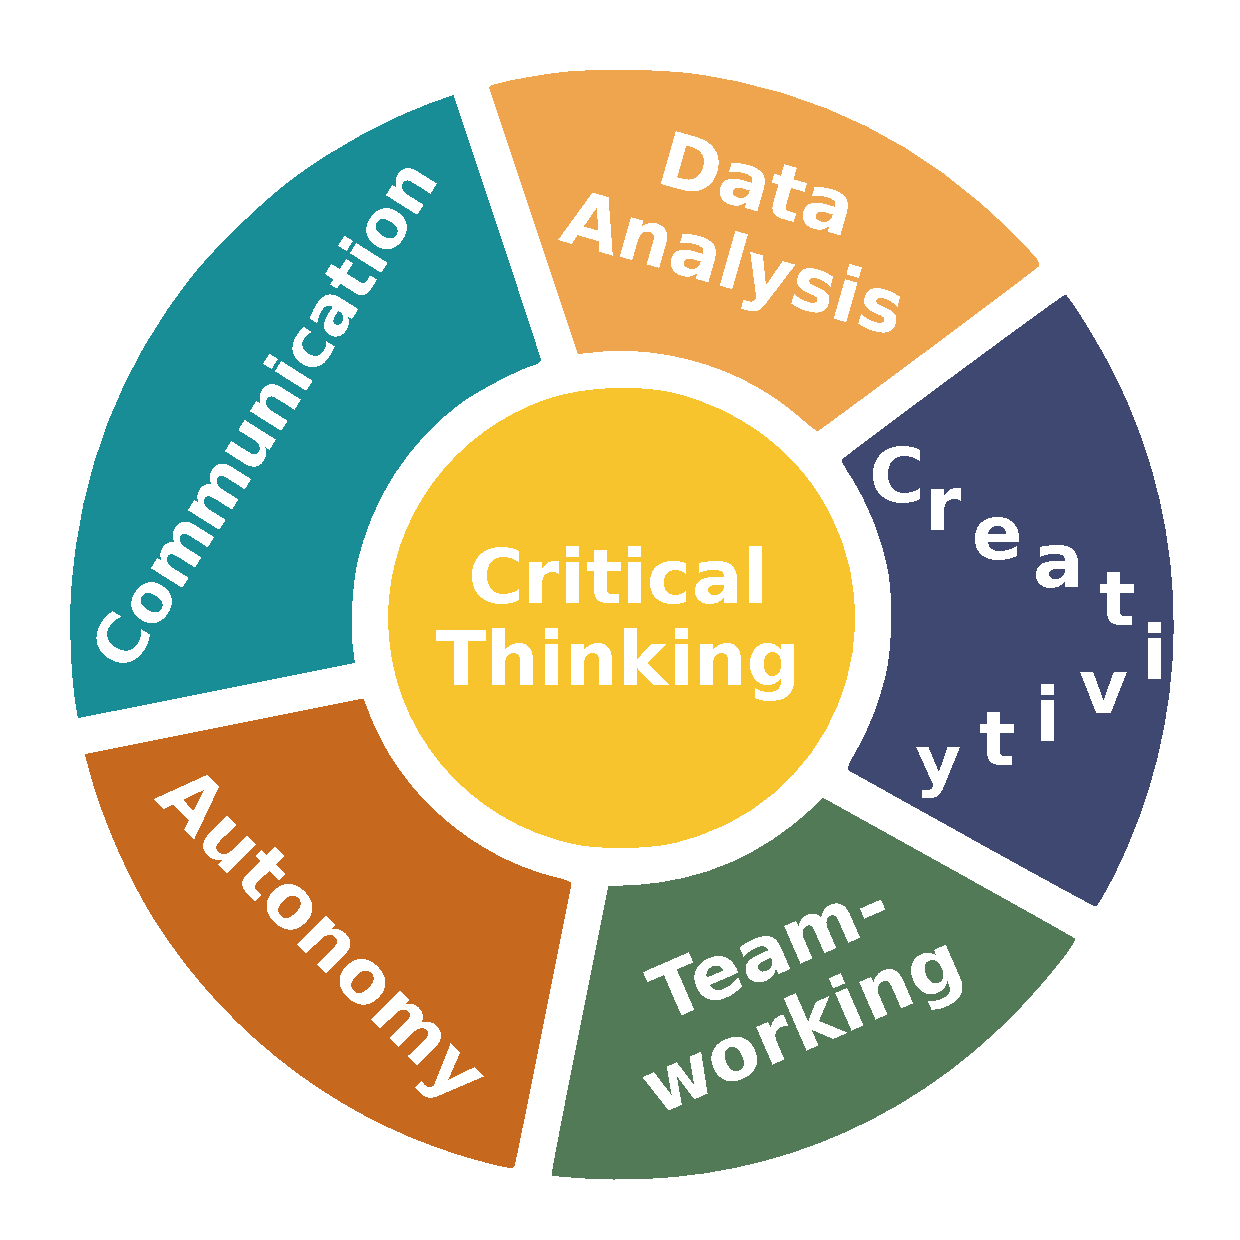
\includegraphics[scale=0.3]{img/skills1.pdf}\\
      \vspace*{4mm}

%   \textcolor{azul}{\bf\Large Language}\\ \vspace*{3mm}
% 
%     {{\bf Spanish:} native }\\%
\includegraphics[width=1.5cm,height=0.27cm]{img/5stars.pdf}\\  %\vspace*{-1mm}
%     {{\bf English:} fluent }%
\includegraphics[width=1.5cm,height=0.22cm]{img/4-8stars.pdf}\\
%     \vspace*{4mm}

  \textcolor{azul}{\bf\Large Technical Skills}\\ \vspace*{4mm}

  \textcolor{azul}{\bf\large \textbullet~~ OS Preference}\\ \vspace*{3mm}

%     {GNU/Linux }
\includegraphics[scale=0.25]{img/5stars.pdf}
    {GNU/Linux }
\includegraphics[width=1.5cm,height=0.27cm]{img/5stars.pdf}\\ %\vspace*{-1mm}
    {Windows }
\includegraphics[width=1.5cm,height=0.22cm]{img/4-8stars.pdf}\\ %\vspace*{-1mm}
    {MacOS }
\includegraphics[width=1.5cm,height=0.19cm]{img/4stars.pdf}\\
    \vspace*{4mm}

   \textcolor{azul}{\bf\large \textbullet~~ Programming}\\ %\vspace*{3mm}
   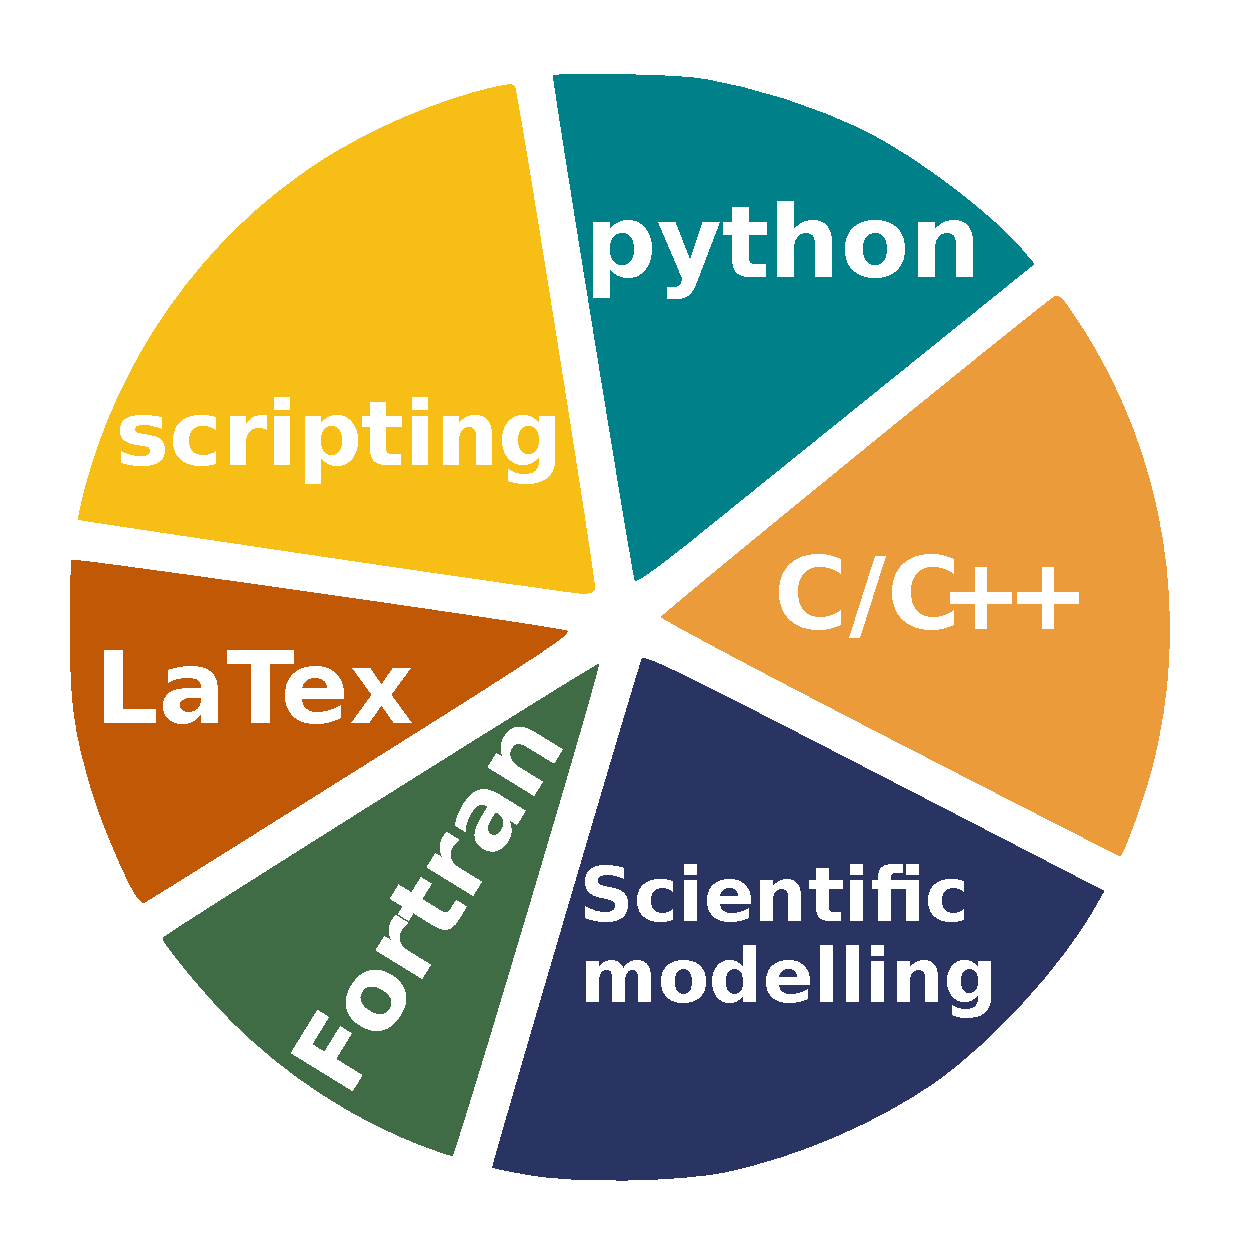
\includegraphics[scale=0.3]{img/programming1.pdf}\\
%      \vspace*{5mm}

 \end{flushright}
\end{minipage}
% }
%--------------------------------------------------------------------------------------------------------
\begin{minipage}{0.1\columnwidth}
%  \textcolor{white}{}
\end{minipage}
\begin{minipage}{0.1\columnwidth}
%  \textcolor{white}{}
\end{minipage}
\begin{minipage}{0.1\columnwidth}
%  \textcolor{white}{}
\end{minipage}
% \begin{minipage}{0.1\columnwidth}
% %  \textcolor{white}{}
% \end{minipage}
%--------------------------------------------------------------------------------------------------------
\begin{minipage}{0.65\columnwidth}

% \vspace*{-6mm}
% \begin{minipage}{0.2\columnwidth}%\vspace*{-3mm}
% % \begin{center}
% % \fcolorbox{   white}{gray!50!white}{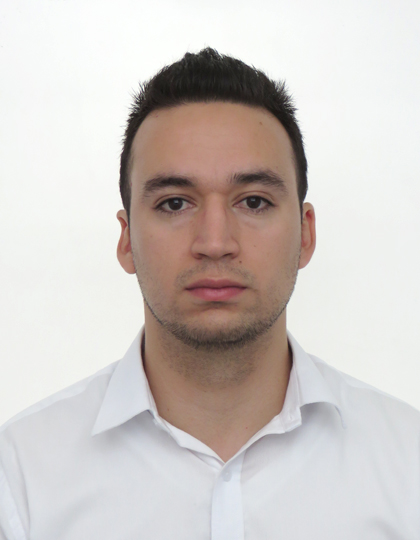
\includegraphics[scale=0.8]{img/EdisonFlorez_1035419798_NZ_visa.jpg}}
% \vspace*{8mm}
% 
\includegraphics[scale=0.1]{img/qr_google_sites.pdf}
% % \end{center}
% \end{minipage}
% \begin{minipage}{0.75\columnwidth}
% \begin{center}
% % {{\fontsize{35}{60}\selectfont Edison\bf Florez}\\[5pt] \textcolor{azul}{\bf\Large Computational Chemist}}
% % \vspace*{-5mm}
% \begin{flushright}
%  {{\fontsize{40}{60}\selectfont Edison\bf Florez}\\[5pt] \textcolor{azul}{\bf\Large Computational Chemist}}
% \end{flushright}
% \end{center}
% \end{minipage}


\vspace*{-5mm}
\begin{flushright}
 {{\fontsize{40}{60}\selectfont Edison\bf Florez}\\[5pt] \textcolor{azul}{\bf\Large Computational Chemist}}
\end{flushright}

\vspace*{-1mm} 
\hspace*{-1.9mm}
\noindent
{\color{gray!20!white} \rule{1.01\linewidth}{3mm} }

%--------------------------------------------------------------------------------------------------------

\vspace*{-5mm}
{\bf\large Profile:}
I want to understand chemistry at its most fundamental level by using computers. Quantum Chemistry is used in a variety of ways to analyze and explain interesting problems of science. In what I do, not only do you learn about chemistry, biology or physics, but you also learn how to use a computer and how to write programs to build models and simulations of real-world processes and systems. The primary goal of my work has been to obtain fundamental insights that are otherwise difficult to obtain by other means.\\
% definitive information which otherwise could not be derived.\\

% \vspace*{-4mm}
% {\small\bf Keywords:}
% {\small Statistical physics $\cdot$ Monte-Carlo methods $\cdot$ phase transitions $\cdot$ potential energy surface $\cdot$ chemical bonding and bond analysis methods $\cdot$ relativistic effects $\cdot$ magnetic field $\cdot$ NMR parameters.}


% Quantum chemistry is today used within all branches of chemistry and molecular physics [and] affords deeper understanding of molecular processes that cannot be obtained from experiments alone.

% Since 1998 the crucial role of theoretical chemistry and computational modelling became more and more evident and nowadays it has become a mandatory tool in the experimental sciences.

% to develop accuracy, improve/scale up reliable models and to get information unavailable otherwise

% The primary goal in the development of general nonperturbative methods in quantum field theories has been the combination of modern computer aided stochastic methods with analytic field theoretic tools to obtain definitive results which otherwise could not be derived.

\vspace*{-2mm}
{\bf\large About me:}
I enjoy a good challenge, big or small, and I firmly believe that given enough time and resources, one achieves any purpose. One of my skills is to hold a long-term focus while executing each step of my plans. I am intuitive and imaginative, open-minded and very resourceful to learn new skills quickly. Aside from science, in my spare time, I am a wine and beer enthusiast, and I am committed to painting, drawing and cycling, not all at the same time. Also, I am a serious/amateur reader (if that is something).

\vspace*{-1mm}
\hspace*{-1.9mm}
\noindent
{\color{gray!20!white} \rule{1.01\linewidth}{3mm} } 
%--------------------------------------------------------------------------------------------------------

\vspace*{-4mm}

% {\bf\Large Personal \textcolor{azul}{Information}}
% \begin{itemize}
% \itemsep-1.5mm
%  \item {\bf Date of birth:}
%  October 22, 1988
%   \item {\bf Nationality:}
%  Colombian
%  \item {\bf ID/Passport: }% / NZ visa:}
%   AN832116
%  \item {\bf NZ visa:}
%   No restrictions on the hours I can work
% %  there are no restrictions on the hours you can work.
% \end{itemize}


\vspace*{1mm}
{\bf\Large Current \textcolor{azul}{Position}}\\ \vspace*{-6mm}

\begin{itemize}
% \itemsep-1mm

  \item {\bf Ph.D. Candidate}\hfill \textcolor{azul}{Since May.2017}

%   {\bf Supervisor:} Dr. Elke Pahl.\\
  {\bf Supervisor:} Distinguished Prof. Peter Schwerdtfeger\\[2mm]
  Centre for Theoretical Chemistry and Physics\\
%   New Zealand Institute for Advanced Study\\
  Massey University (Albany Campus)\\
  Auckland, New Zealand

  {\bf Research:}
  It spans topics in Computational Physics and Chemistry, with an emphasis on computational modelling. In particular, I am interested in the ab initio description of ground state properties of atoms in high magnetic fields and relativistic effects of atomic and molecular systems. Additionally, in the description of phase transitions like melting in nanoclusters and extended systems under strong magnetic fields and understanding the emergence of their bulk properties. I have expertise in the fields of importance-sampling Monte-Carlo, optimization technics, molecular dynamics methods, and electronic structure calculations. 
\end{itemize}

% \vfil
\end{minipage}

% ----------------------------------------------------------------------------------------------------------------------------
\newpage
 
{\bf\Large Professional \textcolor{azul}{Experience}}\\ \vspace*{-6mm}

\begin{itemize}

  \item {\bf Demonstrator:} \hfill \textcolor{azul}{Since Aug.2017}\\
  {Massey University({\href{www.massey.ac.nz}{\textcolor{azul}{\em massey.ac.nz}}}), Auckland, New Zealand} 
  
  \emph{\textbf{Physics:} Teaching and counseling students in workshops with a particular focus on advanced mechanics, thermodynamics, fluids, magnetic fields and electromagnetism, AC circuits.} 

  \item {\bf Lesson Planner and Teacher:}\hfill \textcolor{azul}{Since Feb.2018}\\
  {A\&E International({\href{www.naeaedu.com}{\textcolor{azul}{\em naeaedu.com}}}), Auckland, New Zealand}  

  \emph{\textbf{STEAM:} produce teaching contents for STEAM courses, which correspond to the New Zealand Curriculum. Preparation of course materials for a new class, creation of course material for teaching at school and online. Guide  and counseling students to understand and implement appropriate STEAM projects and workshops.}
  
  \item {\bf Consultant:}\hfill \textcolor{azul}{Aug.2016 - Mar.2017}\\
  {ifb Andina ({\href{www.ifb-group.com/en/}{\textcolor{azul}{\em ifb-group.com}}}), Colombia.}
  
%   \emph{\textbf{SAP Bank-Analyzer:} I have developed complex models, thinking in a cross-system way and analysing economic problems within a customized IT-solution development.}
    
  \emph{\textbf{SAP-Implementation and Bank-Analyzer AFI:} %As a natural scientist,
  develop complex models, thinking in a cross-system way and analyzing economic problems within the development of a customized IT-solution. Also, the development and implementation of mathematical models that relate to economic questions and the attention to detail as well as pragmatic solutions, which help banks and insurance companies to be proactive in the market.}
  
%   you will analyze business and technical methods and use the results to develop solutions tailored to the individual needs of our clients. In general these solutions will be realized predominantly in a SAP or Oracle environment for Analytical Banking, Business Intelligence or planning and consolidation.

  \item {\bf Graduate Teaching Assistant:}\hfill \textcolor{azul}{Sept.2015 - Aug.2016}\\
  {University of Antioquia {\href{www.udea.edu.co}{\textcolor{azul}{\em udea.edu.co}}}, Colombia.}
  
  \emph{\textbf{Quantum Chemistry:} Introduce advanced college students to study of the Quantum Chemistry, getting them to dominate the quantum language, the relevant methods and the concepts, as well as its interpretation and application in systems of chemical interest.}
  
  \emph{\textbf{Chemistry II:} Guide college students through the concepts, methods and theories used in chemistry to represent and describe the structure and the bond of the matter and how it constitutes substances. }
%   Besides, understand and rationalize matter properties at molecular (atomic structure and molecules) and macroscopic level.}
% 
%   \item {\bf Tutor:}\hfill \textcolor{azul}{Feb.2016 - Aug.2016}\\
%   {Grupo Formarte, Colombia.}
% 
%   \emph{\textbf{Basic Science:} Chemistry, Physic and Biology. Teaching and counseling students for understanding and implementing appropriate scientific projects, exams and workshops.} 
%   
\end{itemize}


{\bf\Large Academic \textcolor{azul}{Background}}\\ \vspace*{-6mm}

\begin{itemize}
%  \itemsep-1mm
  \item {\bf Master of Science in Chemistry}\hfill \textcolor{azul}{Jan.2013 - Dec.2014}\\
  Computational Chemistry, University of Antioquia, Colombia\\
%   \emph{\textbf{Thesis:} ``Relativistic Effects in the Microsolvation Process of Methylmercury''.}\\
  {\bf Supervisor:} Prof. Albeiro Restrepo.
%   {\bf Co-supervisors:} Prof. G. Aucar, Prof. J. David and PhD. A. Maldonado
  
  \item {\bf Bachelor of Science in Chemistry}\hfill \textcolor{azul}{Jan.2006 - Jul.2012}\\
  Computational Chemistry, University of Antioquia, Colombia\\
%   \emph{\textbf{Thesis: }``Relativistic Effects in the Molecular Geometry of the XH$_4^+$ Series (X=C, Si, Ge, Sn, Pb)''.}\\
  {\bf Supervisor:} Prof. Albeiro Restrepo.
%   {\bf Co-supervisor:} Prof. J. David  

\end{itemize}

%--------------------------------------------------------------------------------------------------------

% \newpage
{\bf\Large Fellowships \textcolor{azul}{and Awards}}\\ \vspace*{-6mm}

\begin{itemize}
 \itemsep-1mm
  \item {\bf Ph.D. in Physics:} Massey University Doctoral Scholarship for full-time study 2017-2020
  \item {\bf M.Sc. in Chemistry:} Honours and research work with meritorious award.
  \item {\bf B.Sc. in Chemistry:} Honours.  
  
\end{itemize}

%PONER ALGO COMO TRABAJO COLABORATIVO

%{\bf\Large Research \textcolor{azul}{Experience}}\\ \vspace*{-6mm}
%
%\begin{itemize}
% \itemsep-1mm
%
%  \item {\bf Theoretical Chemical Physics Group}\hfill \textcolor{azul}{Since Oct.2010}\\
%  University de Antioquia, Colombia\\
%  \emph{\textbf{Head:} Prof. PhD. Albeiro Restrepo.}\\ \vspace*{-5mm}
%
%  \item {\bf Atomic and Molecular Physic}\hfill \textcolor{azul}{Since Jul.2014}\\
%  Northeastern University, Argentina\\
%  \emph{\textbf{Head:} Prof. PhD. Gustavo Aucar.}\\ \vspace*{-5mm}
%
%\end{itemize}

%%--------------------------------------------------------------------------------------------------------
%
%\newpage


{\bf\Large Supervision \textcolor{azul}{of Theses}}\\ \vspace*{-6mm}

\begin{itemize}
 \item {\bf Co-supervisor M.Sc. thesis, computational chemistry::}\hfill \textcolor{azul}{Sicnce Feb.2018}\\
 \emph{``Microsolvation of Heavy Halides[X(H2O)$_n$]$^-$ (X = Br, I, At; $n=1-6$)''}. \\
 University of Antioquia, Colombia
 
 \item {\bf Co-supervisor B.Sc. thesis, computational chemistry:}\hfill \textcolor{azul}{Nov.2015 - Nov.2017}\\
 \emph{``Relativistic and Electron Correlation Effects on the Calculation of NMR Parameters in M--X Diatomic Molecules (M=Cu, Ag, Au; X=F, Cl, Br, I)''}.\\
 University of Antioquia, Colombia
\end{itemize}


%--------------------------------------------------------------------------------------------------------

{\bf\Large Peer--reviewed \textcolor{azul}{Publications}}\\ \vspace*{-6mm}

\begin{itemize}
%  \itemsep-1mm

  \item {\bf Edison Florez}, Alejandro Maldonado, Gustavo Aucar, Jorge David y Albeiro Restrepo. \emph{``Microsolvation of Methylmercury: Structures, Energies, Bonding and NMR Constants ($^{199}$Hg, $^{13}$C and $^{17}$O)''}. {\em Phys. Chem. Chem. Phys.} {\bf 2016}, 18, 1537-1550. \underline{DOI: 10.1039/c5cp04826e}

  \item Yuly Chamorro, {\bf Edison Florez}, Alejandro Maldonado, Gustavo Aucar, and Albeiro Restrepo. \emph{``Microsolvation of heavy halides. Int J Quantum Chem''}. {\bf 2020}; e26571. \underline{DOI: 10.1002/qua.26571}

  \item {\bf Edison Florez}, Trygve Helgaker, Wim~Klopper, Peter~Schwerdtfeger, Andrew~Teale, Stella Stopkowicz, Elke~Pahl. \emph{``Melting of Neon in High Magnetic Fields''}. \underline{In preparation}  

%   \item Yuly Chamorro, Alejandro Maldonado, {\bf Edison Florez}, Gustavo Aucar, and Albeiro Restrepo. \emph{``Relativistic and Electron Correlation Effects on the Calculation of NMR Parameters in M--X Diatomic Molecules (M=Cu, Ag, Au; X=F, Cl, Br, I)''}. \underline{Submitted}
  
\end{itemize}

%--------------------------------------------------------------------------------------------------------

{\bf\Large Reviewer \textcolor{azul}{Activities}}\\ \vspace*{-6mm}

\begin{itemize}

  \item {\bf INGE CUC:} {\small\em Printed ISSN: 0122-6517 and Electronic ISSN: 2382-4700}. Journal of the Faculty of Engineering of the Universidad de la Costa, Barranquilla, Colombia. 

\end{itemize}

%--------------------------------------------------------------------------------------------------------
% \newpage

% {\bf\Large Scientific \textcolor{azul}{Events}}\\ \vspace*{-6mm}
% 
% \begin{itemize}
% \itemsep-1mm
% 
%  \item {\bf Microsolvation of Methylmercury (CH$_3$Hg$^+$): structures, energies, bonding and NMR constants ($^{199}$Hg, $^{13}$C and $^{17}$O)}\vspace*{-3mm}
%  
%   \begin{itemize}
%    \itemsep-1mm
%    \item \emph{International Conference on Relativistic Effects in Heavy-Elements (REHE 2014). Septiembre 20 al 24 de 2014. Smolenice Castle, Slovak Republic.} \underline{\bf Poster}    
%    \item \emph{V National Meeting of Theoretical and Computational Chemists (V-ENQTC). April 27-30, 2014. Guatapé, Antioquia, Colombia.} \underline{\bf Poster}
%   \end{itemize}  
%   
%   \item {\bf Relativistic Effects in the Molecular Geometry of Cationic Methane}\vspace*{-3mm}
%  
%   \begin{itemize}
%    \item \emph{V National Meeting of Theoretical and Computational Chemists (V-ENQTC). April 27-30, 2014. Guatapé, Antioquia, Colombia.} \underline{\bf Poster}
%   \end{itemize}
% 
%  \item {\bf Relativistic Effects in the Molecular Geometry of XH$_4^+$ serie (X=C, Si, Ge, Sn and Pb)}\vspace*{-3mm}
%  
%   \begin{itemize}
%    \itemsep-1mm
%    \item \emph{International Conference on Relativistic Effects in Heavy-Elements (REHE 2012). Septiembre 12 al 16 de 2012. Northeastern University, Corrientes, Argentina.} \underline{\bf Poster}    
%    \item \emph{IV National Meeting of Theoretical and Computational Chemists (IV-ENQTC). April 28-31, 2012. University of Valle, Cali, Colombia.} \underline{\bf Poster}
%   \end{itemize}
%   
% \end{itemize}
% 
% \hspace*{5mm}
% {\bf\large As \textcolor{azul}{Co-author}}\\ \vspace*{-6mm}
% 
% \begin{itemize}
% \itemsep-1mm
% 
%  \item {\bf Relativistic and Electron Correlation Effects on the Calculation of NMR Parameters in M--X Diatomic Molecules (M=Cu, Ag, Au; X=F, Cl, Br, I)}  \underline{Yuli Chamorro}, Edison Flórez, Alejandro Maldonado, Jorge David, Gustavo Aucar and Albeiro Restrepo. \vspace*{-3mm}
% 
%   \begin{itemize}
%    \itemsep-1mm
%    \item \emph{VI National Meeting of Theoretical and Computational Chemists (VI-ENQTC). September, 2016. Universidad Nacional de Colombia, Bogotá D.C., Colombia.} \underline{\bf Poster}
%   \end{itemize}
%   
% \end{itemize}

%--------------------------------------------------------------------------------------------------------

%\newpage


%{\bf\Large Complementary \textcolor{azul}{Formation}}\\ \vspace*{-6mm}
%
%\begin{itemize}
% \itemsep-1mm
%
%  \item {\bf Course:} Magnetism in Nanostructured Materials.\\
%  \emph{Lecturer: PhD. Francisco Homero Sánchez (Argentina)}. November 2012. Universty EAFIT, Medellín, Colombia.
%
%  \item {\bf Course:} Fundamentals of Quantum Electrodynamics and Applications to Atomic Systems.\\
%  \emph{Lecturer: PhD. Jonathan Sapirstein (USA) and PhD. Vladimir Shabaev (Russia)}. September 2012. Northeastern University, Corrientes, Argentina.
%
%  \item {\bf Course:} Introduction to Relativistic Quantum Chemistry and Molecular Physics.\\
%  \emph{Lecturer: PhD. Kenneth Dyall (USA), PhD. Hans Joergen Jensen (Denmark) and PhD. Stefan Knecht (Denmark)}. September 2012. Northeastern University, Corrientes, Argentina.
%
%\end{itemize}

%--------------------------------------------------------------------------------------------------------

\vspace*{2mm}
{\bf\Large Refer\textcolor{azul}{ences}}\\
(Available upon request)

% \begin{itemize}
%  \itemsep-1mm
% 
%   \item {\bf Prof. PhD. Albeiro Restrepo Cossio}\\
%   Professor University of Antioquia. Medellín, Colombia.\\
%   Head of Theoretical Chemical Physics Group.\\
%   albeiro.restrepo@udea.edu.co\\
%   Telephone: +57 320 603 1603\\ \vspace*{-3mm}
% 
%   \item {\bf Prof. PhD. Gustavo Adolfo Aucar}\\
%   Profesor Universidad Nacional del Nordeste, Corrientes, Argentina.\\
%   Head of Institute of Modeling and Innovation Technological (IMIT), CONICET.\\ 
%   gaa@unne.edu.ar\\
%   Telephone: +54 (0) 376 (15) 430 7839\\ \vspace*{-3mm}
% 
% \end{itemize}

%--------------------------------------------------------------------------------------------------------
\vfill
% {\vspace*{-4mm}\hfill $\blacksquare$}

\begin{flushright}
 \href{https://sites.google.com/view/edisonflorez/home}{
\includegraphics[scale=0.15]{img/qr_google_sites.pdf}}
\end{flushright}

\vspace*{5mm}
 Auckland, New Zealand\\
 \today

\vfill

\begin{flushright}
 Your sincerely,\\ \vspace*{4mm} 
  
\includegraphics[scale=0.23]{img/firma.pdf}\\ \vspace*{-10mm}  
 -----------------------------------\\
 M.Sc. Edison Flórez %\\
%  \today\\
%  Auckland, NZ.
 
\end{flushright}

\end{document}
